% Generated by code/needham.py -- do not edit by hand.
\definecolor{qocA}{rgb}{0.00,0.45,0.70}
\definecolor{qocB}{rgb}{0.90,0.60,0.00}
\definecolor{qocC}{rgb}{0.00,0.62,0.45}
\definecolor{qocD}{rgb}{0.80,0.40,0.00}
\definecolor{qocE}{rgb}{0.80,0.60,0.70}
\definecolor{qocF}{rgb}{0.35,0.70,0.90}
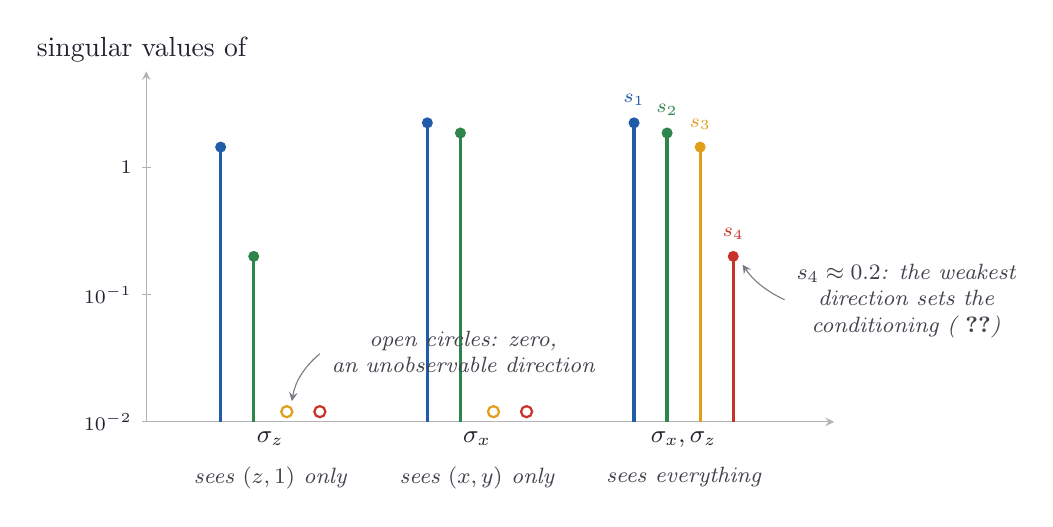
\begin{tikzpicture}[ink/.style={line width=0.9pt, ndInk}, faint/.style={line width=0.4pt, ndInk!35}, dashedink/.style={line width=0.5pt, ndInk!55, dash pattern=on 2.5pt off 2pt}, vec/.style={->, >=stealth, line width=1.2pt}, note/.style={font=\footnotesize\itshape, text=ndInk!85, align=center}, pointer/.style={->, >=stealth, line width=0.4pt, ndInk!60, shorten >=2pt, shorten <=1pt}, dot/.style={circle, fill=ndInk, inner sep=0pt, minimum size=3.4pt}, wash/.style={fill=ndSky, fill opacity=0.55}, every node/.style={text=ndInk}]
\definecolor{ndInk}{rgb}{0.13,0.13,0.18}
\definecolor{ndPaper}{rgb}{0.99,0.96,0.88}
\definecolor{ndSky}{rgb}{0.84,0.91,0.98}
\definecolor{ndRose}{rgb}{0.98,0.86,0.84}
\definecolor{ndBlue}{rgb}{0.13,0.36,0.66}
\definecolor{ndRed}{rgb}{0.78,0.20,0.16}
\definecolor{ndGold}{rgb}{0.88,0.62,0.10}
\definecolor{ndGreen}{rgb}{0.18,0.52,0.30}
\draw[faint, ->, >=stealth] (0.000,0.000) -- (8.736,0.000) node[right, text=ndInk] {};
\draw[faint, ->, >=stealth] (0.000,0.000) -- (0.000,4.452) node[above, text=ndInk] {singular values of $\Obsv$};
\draw[faint] (0.060,0.000) -- (-0.060,0.000) node[left, font=\scriptsize, text=ndInk] {$10^{-2}$};
\draw[faint] (0.060,1.615) -- (-0.060,1.615) node[left, font=\scriptsize, text=ndInk] {$10^{-1}$};
\draw[faint] (0.060,3.231) -- (-0.060,3.231) node[left, font=\scriptsize, text=ndInk] {$1$};
\draw[line width=1.2pt, ndBlue] (0.945,0.000) -- (0.945,3.489);
\fill[ndBlue] (0.945,3.489) circle (2pt);
\draw[line width=1.2pt, ndGreen] (1.365,0.000) -- (1.365,2.101);
\fill[ndGreen] (1.365,2.101) circle (2pt);
\draw[line width=0.8pt, ndGold, fill=white] (1.785,0.129) circle (2pt);
\draw[line width=0.8pt, ndRed, fill=white] (2.205,0.129) circle (2pt);
\node[below, font=\small] at (1.575,0.000) {$\sigma_z$};
\node[note, below] at (1.575,-0.450) {sees $(z,1)$ only};
\draw[line width=1.2pt, ndBlue] (3.570,0.000) -- (3.570,3.797);
\fill[ndBlue] (3.570,3.797) circle (2pt);
\draw[line width=1.2pt, ndGreen] (3.990,0.000) -- (3.990,3.668);
\fill[ndGreen] (3.990,3.668) circle (2pt);
\draw[line width=0.8pt, ndGold, fill=white] (4.410,0.129) circle (2pt);
\draw[line width=0.8pt, ndRed, fill=white] (4.830,0.129) circle (2pt);
\node[below, font=\small] at (4.200,0.000) {$\sigma_x$};
\node[note, below] at (4.200,-0.450) {sees $(x,y)$ only};
\draw[line width=1.2pt, ndBlue] (6.195,0.000) -- (6.195,3.797);
\fill[ndBlue] (6.195,3.797) circle (2pt);
\draw[line width=1.2pt, ndGreen] (6.615,0.000) -- (6.615,3.668);
\fill[ndGreen] (6.615,3.668) circle (2pt);
\draw[line width=1.2pt, ndGold] (7.035,0.000) -- (7.035,3.489);
\fill[ndGold] (7.035,3.489) circle (2pt);
\draw[line width=1.2pt, ndRed] (7.455,0.000) -- (7.455,2.101);
\fill[ndRed] (7.455,2.101) circle (2pt);
\node[below, font=\small] at (6.825,0.000) {$\sigma_x,\sigma_z$};
\node[note, below] at (6.825,-0.450) {sees everything};
\node[note, anchor=west] (z) at (2.231,0.888) {open circles: zero,\\ an unobservable direction};
\draw[pointer] (z.west) to[bend right=20] (1.838,0.194);
\node[note, anchor=west] (s) at (8.138,1.535) {$s_4\approx0.2$: the weakest\\ direction sets the\\ conditioning (\Chap~\ref{C.SampleComplexity})};
\draw[pointer] (s.west) to[bend left=15] (7.534,2.053);
\node[font=\scriptsize, text=ndBlue] at (6.195,4.087) {$s_1$};
\node[font=\scriptsize, text=ndGreen] at (6.615,3.958) {$s_2$};
\node[font=\scriptsize, text=ndGold] at (7.035,3.779) {$s_3$};
\node[font=\scriptsize, text=ndRed] at (7.455,2.392) {$s_4$};
\end{tikzpicture}
